\documentclass{CFD2015}
\usepackage{CFD2015}

%%%%%%%%%%%%%%%%%%%%%%%%%%%%%%%%%%%%%%%%%%%%%%%%%%%%%%%%%%%%%%%%%%%%%%%%%
%This template is created for complying with the author instructions for the 
%8th International Conference on CFD in Oil & Gas, Metallurgical and Process Industries
%hosted by SINTEF/NTNU, Trondheim Norway
%17-19 June 2015
%
%Sverre G. Johnsen (sverre.g.johnsen@sintef.no)
%SINTEF Materials and Chemistry


%Required files:
%   ExampleFile.tex
%   ExampleFile.nls
%   CFD2015.bst
%   CFD2015.cls
%   CFD2015.sty
%   References.bib

%Example-specific files:
%   figure.eps
%   Table.tex
%%%%%%%%%%%%%%%%%%%%%%%%%%%%%%%%%%%%%%%%%%%%%%%%%%%%%%%%%%%%%%%%%%%%%%%%%




\title{Establishing the predictive capabilities of DEM simulations: sliding and rolling friction coefficients of non-spherical particles}
\paperID{CFD 2015}
\author{Luca}{Benvenuti} %{forename}{surname}
\presenting  %the previous author is presenting the paper (name becomes underlined)
\address{JKU Department of Particulate Flow Modelling, 4040 Linz, Austria} %affiliation of the previous author
\email{luca.benvenuti@jku.at}%e-mail address of the previous author
\author{Andreas}{Aigner}
\sameaddressas{1}
%\email{andreas.aigner@jku.at}
\author{Daniel}{Queteschiner}
\sameaddressas{1}
%\email{daniel.queteschiner@jku.at}
\author{Mar}{Combarros}
\address{TUBS Institut fur Partikeltechnik, 38104 Braunschweig, Germany} %same address as the first author
%\email{m.combarros-garcia@tu-braunschweig.de}
\author{Stefan}{Pirker}
\sameaddressas{1}
%\email{stefan.pirker@jku.at}
\author{Christoph}{Kloss}
\sameaddressas{1}
%\email{christoph.kloss@jku.at}


\begin{document}
\maketitle  %create the title page
\headers   %create the page headers and footers


\abstract{
Discrete Element Method ($DEM$) simulations are widely used to understand particle behavior. Among the key parameters, defining the inter-particle friction parameters is very relevant to perform simulations of granular flows.
To model non-spherical particles with spherical elements, we used an elasto-plastic rolling friction model in combination with Coulomb's law in the $DEM$ code LIGGGHTS.
The bulk solids were characterized using Schulze ring shear cell and simplified Jenike shear cell testers. 
The sliding and rolling friction coefficients were obtained by fitting numerical simulations of the shear cells to experimental data.
The calculated DEM coefficients of friction of iron ore, limestone and silibeads accord well with published data and in-house experiments. 
Further, we validated the DEM parameters by means of angle-of-repose experiments and simulations and conclude that the described setup successfully defined the DEM parameters for the materials tested.
}
\keywords{
Meshless methods (DEM), Rheology, experimental validation studies, process industries, process metallurgy, LIGGGHTS, Material characterization 
}
\normalfont\normalsize

%\section{Nomenclature}
%A complete list of symbols used, with dimensions, is required.
%the nomenclature needs to be entered into the file ExampleFile.nls
\printnomenclature[0.7cm]  
\vskip .1em

\section{Introduction}
Particles in various forms - ranging from raw materials to food grains and pharmaceutical powders - play a major role in a variety of industries, including process industry and metallurgy. In his book, \citet{RefWorks:117} stated that "between 1 and 10\% of all the energy is used in comminution, i.e. the processes of crushing, grinding, milling, micronising". 
However, a univocal method to characterize these particles has so far not been established.
%reached yet since the results obtained through experiments could be biased. 
From the experimental point of view, the main issues are the difficult setups and the general reliability and reproducibility of the tests. 
From the numerical point of view, no general procedure is available, and the existence of a mathematically unique solution describing macro/micro particle contact has yet to be proved.
Moreover, in a recent study, \citet{RefWorks:56} implied "that the dynamic properties of a powder cannot be applied to universally predict the static properties of a powder, and, likewise, the static properties cannot be used to predict dynamic properties".\\
Discrete Element Method (DEM) simulations are widely used to understand particle behavior.
\citet{RefWorks:135} defined the $DEM$ as "a special class of numerical schemes for simulating the behavior of discrete, interacting bodies".
The force that particle i exerts on particle j is defined as:
% \ref{equ:newtonlaw}:
\begin{equation}
m \ddot{x}_{ij} + c \dot{x}_{ij} + k x_{ij} =  F_{ij} .
\label{equ:newtonlaw}
\end{equation}
Further details on the method can be found in \citet{RefWorks:133}.
$LIGGGHTS$ (LAMMPS improved for general granular and granular heat transfer simulations) is one of the most powerful open source $DEM$ simulation software packages available. 
The models it can analyze are described in detail in the literature \cite{RefWorks:136}.\label{par:overviewdemliggghts}
In combination with shear cell tester simulation \cite{RefWorks:139}, $LIGGGHTS$ has correctly defined the coefficient of sliding friction for coarse round particles - 
a critical parameter describing inter-particle friction in medium to dense granular flows simulations.\\
Since the bulk solid is represented by perfect spheres, the only parameter the software uses to describe its shape is the radius of the particle ($R$).
However, since the shape is one of the most relevant aspects defining particle behavior, we consider the coefficient of rolling friction ($\mu_r$) as an additional $DEM$ shape parameter. 
It is proportional to the torque counteracting the rotation of the particle and defined as (Eq. \ref{equ:mur}):
\begin{equation}
 \mu_r =  \tan(\iota) .
\label{equ:mur}
\end{equation}
$DEM $ simulations have recently been used to reduce the bias of the experiments, and more precise devices such as the Schulze ring shear cell tester (SRSCT)(see \citet{RefWorks:104}) have been built.
A dedicated workflow that combines experiments and simulations must now be devised following the Design of Experiments method, as illustrated by \citet{RefWorks:116}.\\
The main goal of this new procedure should be the characterization of non-spherical particles, especially the $DEM$ coefficients of friction, following standardizable steps.
With this objective in mind, we profited from the shear cell experimental and numerical setup in combination with $LIGGGHTS$ simulation to improve the accuracy and the range of applicability of particle characterization.
%The aforementioned software $LIGGGHTS $ was used for the simulations.
Since this study was supported by the metallurgical industry, the materials examined were: silibeads (2 mm), coke, iron ore, limestone (all 0-3.15 mm).\\ \label{par:materials}

\section{Model Description}
 \label{sec:modeldesrip}
For the raw materials used in this work \citet{RefWorks:145} suggested using the non-linear Hertzian model without cohesion for the particle-particle and particle-wall contacts.\\
This granular model uses the following formula for the force between two granular particles (Eq. \ref{eq:forceij}):
\small
\begin{equation}
 F_{ij} = 
\begin{cases}
F_{n,ij} + F_{t,ij} = \left( k_n \delta_{n,ij} + \gamma_n v_{n,ij} \right) + \left( k_t \delta_{t,ij} + \gamma_t v_{t,ij} \right) & \text{if } r < d ,\\
0    & \text{if } r > d ,\\
\end{cases}
 \label{eq:forceij}
\end{equation}
\normalsize

while the tangential force component is truncated to fulfill

\begin{equation}
F_{t,ij} \leq \mu_s F_{n,ij}.
 \label{eq:force_t}
\end{equation}

Both the normal and the tangential force comprise two terms, a spring force and a damping force. The shear force is a "history" effect that accounts for the tangential displacement ("tangential overlap") between the particles for the duration of contact. \\

The $k_n$, $k_t$, $\gamma_n$, and $\gamma_t$ coefficients are calculated from the material properties as follows:
\begin{equation}
\begin{aligned}
	k_n &= \frac{4}{3} E_{eq} \sqrt{R_{eq} \delta_n} ,\\
	\gamma_n &= 2 \sqrt{\frac{5}{6}} \beta \sqrt{S_n m_{eq}} ,\\
	k_t &= 8 G_{eq} \sqrt{R_{eq}} \delta_n ,\\
	\gamma_t &= 2 \sqrt{\frac{5}{6}} \beta \sqrt{S_t m_{eq}} .
\end{aligned}
\label{eq:hertz}
\end{equation}
%
In addition to the equations \ref{eq:hertz} the following relations (Eqns. \ref{eq:equivProp2}) are required:
%
\begin{equation}
\begin{aligned}
 \frac{1}{E_{eq}} & = \frac{1-\nu_i^2}{E_i} + \frac{1-\nu_j^2}{E_j} ,\\
 \frac{1}{G_{eq}} & = \frac{2(2+\nu_i)(1-\nu_i)}{E_i} + \frac{2(2+\nu_j)(1-\nu_j)}{E_j} ,\\
 \frac{1}{R_{eq}} &= \frac{1}{R_i} + \frac{1}{R_j} ,\\
 \frac{1}{m_{eq}} &= \frac{1}{m_i} + \frac{1}{m_j} ,\\
 \beta & = \frac{\ln(e)}{\sqrt{ln^2(e)+\pi^2}} ,\\
 S_n & = 2 E_{eq} \sqrt{R_{eq} \delta_n} ,\\
 S_t & = 8 G_{eq} \sqrt{R_{eq} \delta_n} ,\\
 k_r & = k_t R_{eq}^2 .\\
\end{aligned}
\label{eq:equivProp2}
\end{equation}

The $\mu_r$ parameter enters the equations according to the elasto-rolling resistance model presented by \citet{RefWorks:87} and \citet{RefWorks:131}, also used by \citet{RefWorks:147}, based on the work of \citet{RefWorks:143}(and in contrast to \citet{RefWorks:144}). The model is called EPSD2 in LIGGGHTS.
This is appropriate for the one way rolling cases as well as the cycling rolling ones.
The total rolling resistance torque is (Eq. \ref{eq:mrtm}):

\begin{equation}
\begin{aligned}
M_r &= M_r^k ,\\
M_{r,ti+\Delta ti}^k &= M_{r,ti}^k - k_r \Delta \theta_r ,\\
\lvert{M_{r,ti+\Delta ti}^k}\rvert & \leq M_r^m = \mu_r R_{eq} F_n .\\
\end{aligned}
 \label{eq:mrtm}
\end{equation}


Given these equations, completely defining a dry material for DEM simulations requires these data:
\begin{itemize}
\item{the radius of the particles ($R$);}
\item{the Young's modulus ($E$) and the Poisson's coefficient ($\nu$);}
\item{the particle density ($\rho_p$) and the coefficient of restitution ($e$);}
\item{the coefficients of sliding ($\mu_s$) and rolling ($\mu_r$) friction.}
\end{itemize}


\section{Experimental setup}
The first step of the procedure was using shear testers - 
a simplified Jenike shear cell tester ($JSCT$, see \citet{RefWorks:114}) and a SRSCT (see \citet{RefWorks:142})
to characterize particle flow properties, especially the complete yield locus.
Each experiment was performed on a fresh material sample. \\
In the tests with the simplified $JSCT$, a representative sample of bulk solid was placed in a shear cell of 104 mm diameter. 
This specimen was pre-consolidated by twisting the shear cell cover while applying a compressive load (from 0.488 to 1.379 kg) normal to it.
Since this was a simplified tester, the specimen was then sheared with the same normal load at a constant velocity. 
In fact, the \textit{shear to failure} phase was missing in these \textit{simplified} tests, and the \textit{consolidation} phase was not completely serialized.
The steady-state flow horizontal stress (Fig. \ref{fig:04sjsctdiagram}) is called pre-shear stress ($\tau_{psh}$). Knowing the normal stress, it gives (Eq. \ref{eq:phi_ps}) the angle of internal friction of the pre-shear phase ($\phi_{e-psh}$), our first flowability value \cite{RefWorks:118}:
\begin{equation}
\begin{aligned}
\phi_{e-psh} &= \arctan \left(\frac{\tau_{psh}}{\sigma_{n,psh}} \right) ,\\
\mu_{psh} &=\tan(\phi_{e-psh}) .
\end{aligned}
 \label{eq:phi_ps}
\end{equation}

\begin{figure}[!htb] 
\centering 
\includegraphics[width=.7\columnwidth]{03sjsct} 
\caption[simplified JSCT]{Jenike shear cell tester \cite{RefWorks:118}}
\label{fig:03sjsct} 
\end{figure}

\begin{figure}[!htb] 
\centering 
\includegraphics[width=.7\columnwidth]{04sjsctdiagram} 
\caption[Sjsct diagram]{Jenike shear cell tester diagram \cite{RefWorks:118}}
\label{fig:04sjsctdiagram} 
\end{figure}

Analogously, in the $SRSCT$ tests a representative sample of bulk solid was placed in a shear cell of specified dimensions ($external ~ radius = 100 ~ mm$, $internal ~ radius = 50 ~ mm$). A normal load was applied to the cover, and the specimen was pre-sheared  until a steady-state shear value was reached, again obtaining $\phi_{e-psh}$. 
The normal stress and the angular velocity were then immediately reduced to zero. 
Subsequently, the specimen was sheared under a fraction of the first normal load until the shear force reached a maximum and began to decrease. Both the pre-shear and shear phases were executed at constant velocity. We define the horizontal stress during the shear force peak as maximum shear stress, thus obtaining (Eq. \ref{eq:phi_s})\cite{RefWorks:118}:
\begin{equation}
\begin{aligned}
\phi_{e-sh} &= \arctan \left(\frac{\tau_{sh}}{\sigma_{n,sh}} \right) ,\\
\mu_{sh} &= \tan(\phi_{e-sh}) .
\end{aligned}
 \label{eq:phi_s}
\end{equation}
From three to four different pre-shear normal loads were applied in the experiment. For each we used
a proportional shear increasing from stage one (40\%) to stage four (100\%) with two escalating intermediate stages (60\% and 80\%).
%with one to four proportional shear normal load each (40\%, 60\%, 80\%, 100\%).
The $\phi_{e-psh}$ values for the limestone obtained with the $SRSCT$ and the simplified $JSCT$ were in good accordance (less than 1\% difference), therefore we were able to validate the latter experimental device for this material.\\

\begin{figure}[!htb] 
\centering 
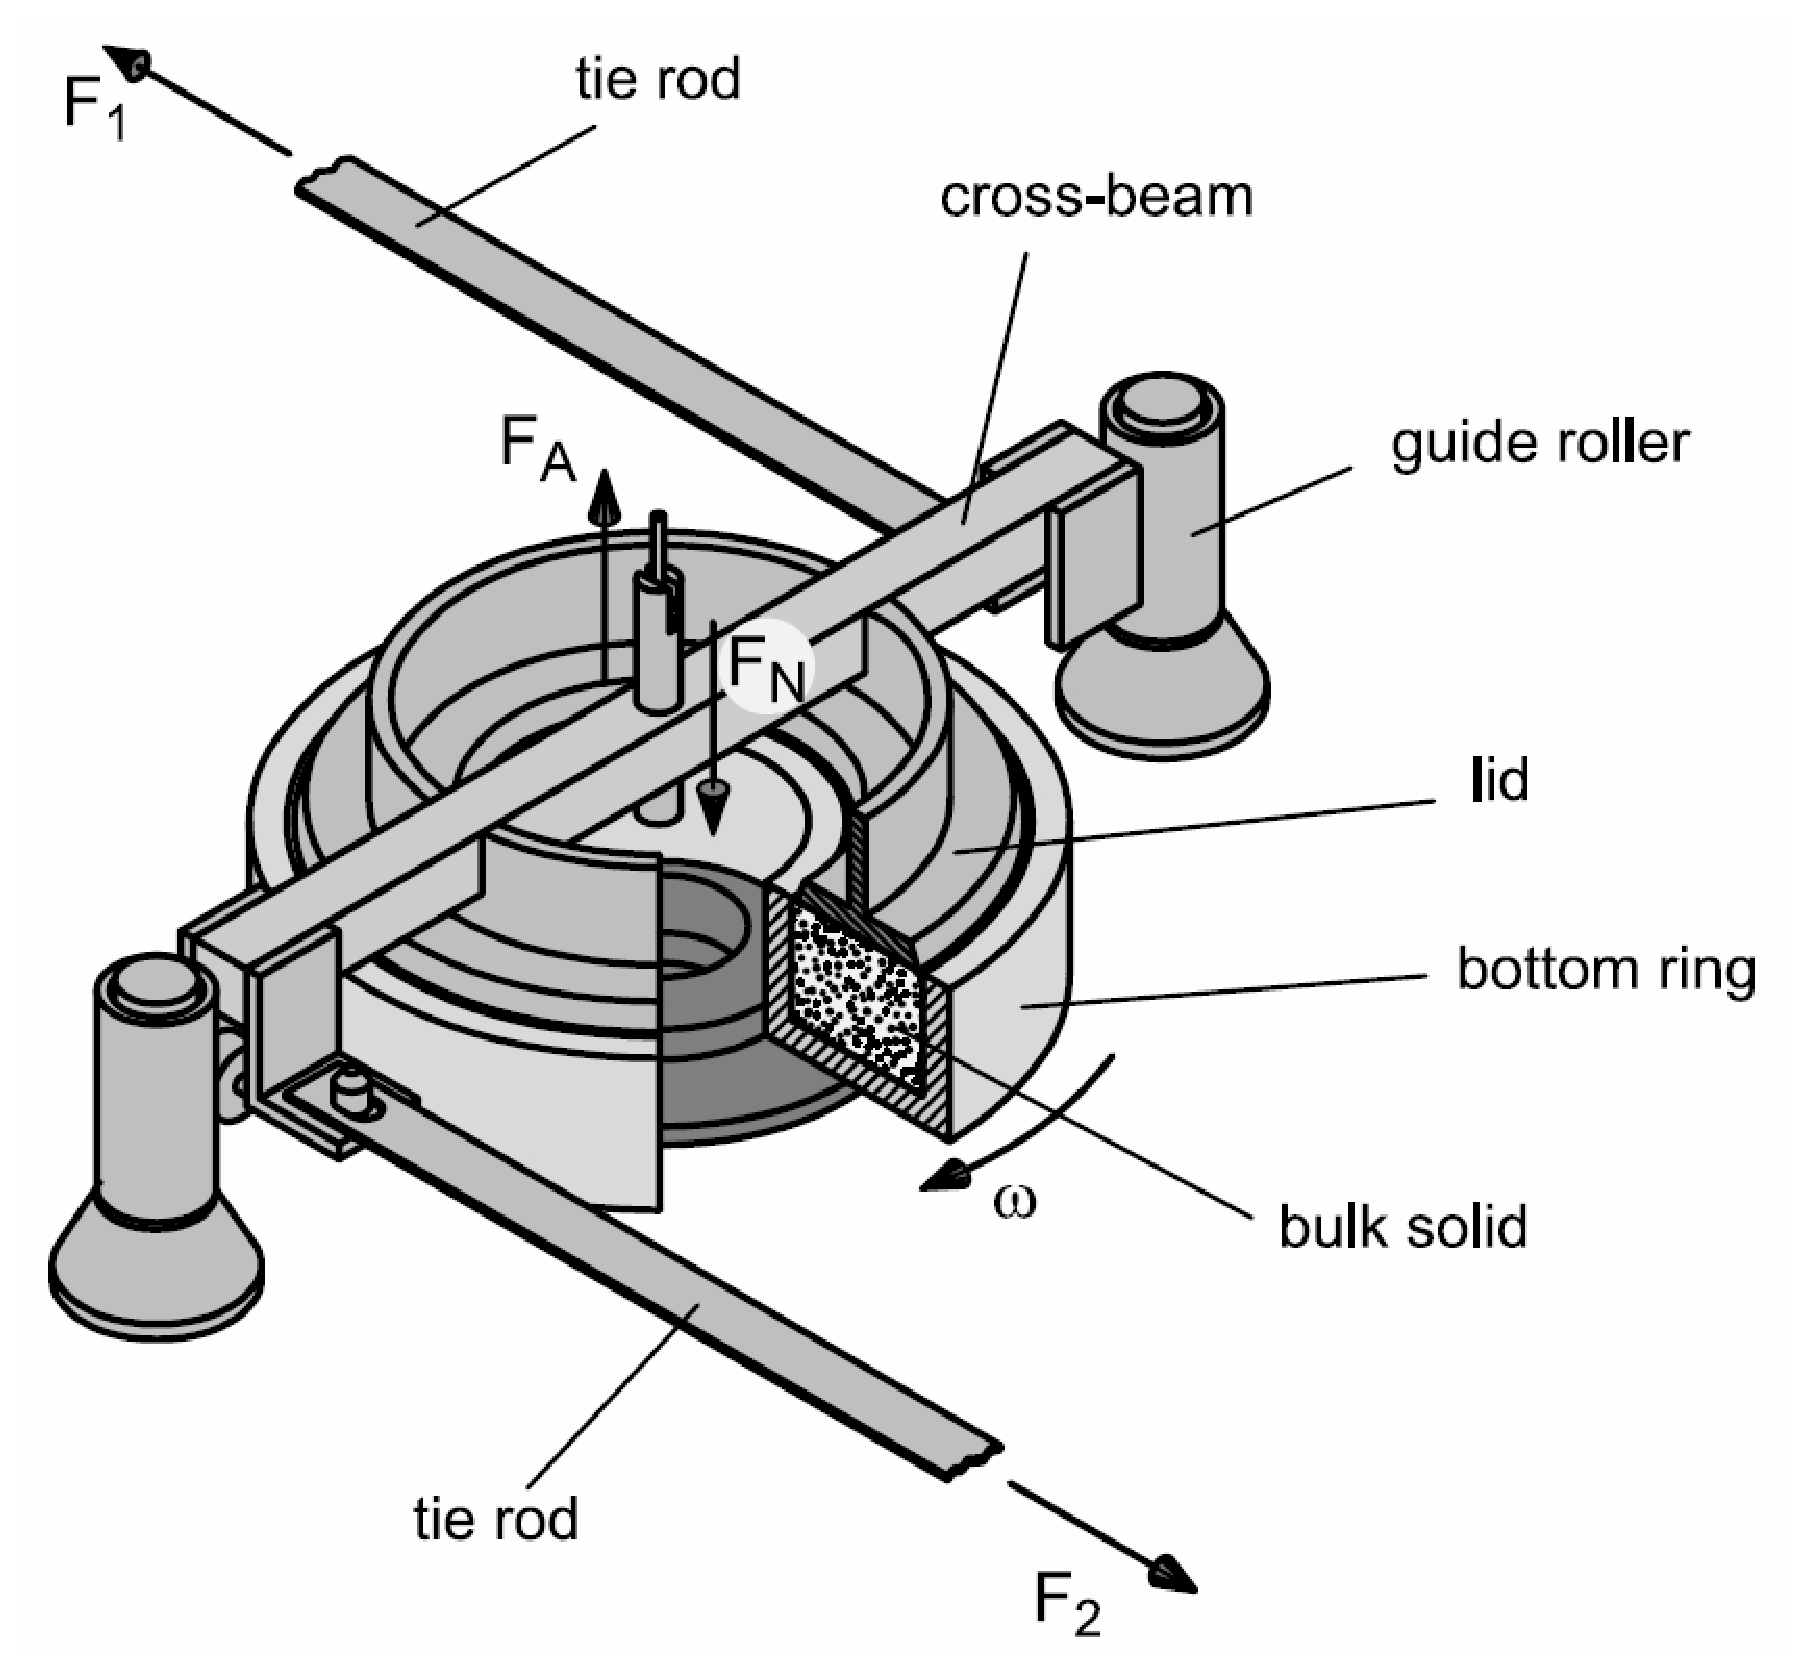
\includegraphics[width=.7\columnwidth]{01srsct} 
\caption[Srsct]{Schulze ring shear cell tester \cite{RefWorks:118}}
\label{fig:01srsct} 
\end{figure}

\begin{figure}[!htb] 
\centering 
\includegraphics[width=.7\columnwidth]{02srsctdiagram} 
\caption[Srsct diagram]{Schulze ring shear cell tester diagram \cite{RefWorks:118}}
\label{fig:02srsctdiagram} 
\end{figure}

\begin{figure}[!htb] 
\centering 
\includegraphics[width=.5\columnwidth]{05aor} 
\caption[Aort]{Angle of repose tester \cite{RefWorks:118}}
\label{fig:05aor} 
\end{figure}

Furthermore, in order to recreate the repose angle observed in a pile of the real material, a sample was deposited on a 20 cm diameter plate with liftable boundary, called static angle of repose ($AOR$) tester (Fig. \ref{fig:05aor}). 
Once the particles were in position, the boundary was lifted, allowing some particles to drop. Once stabilized, the $AOR$ was measured eight times using a digital protractor at different positions of the heap. The result is given as the average of the measurements (Tab. \ref{tab:comparisontable}).\\



\section{Simulations}

$LIGGGHTS$, the simulation toolbox we used, meets most of the requirements of modelling the shear tester described above. First, it is capable of importing triangulated meshes of the two rings and a top lid. Since the real set-up had a wall thickness, both rings have additional horizontal walls that prevent the particles from falling out of the shear cell. Further, all particle-wall contact forces acting on a mesh are summed and can be saved, and thus shear force calculation is available out of the box. Moreover, the code can move a mesh with constant velocity as required for the measurement. 
To determine the shear stresses, the bulk solid had to be stressed with user-defined normal stresses.
Therefore, a stress-controlled wall ($servo-wall$ in $LIGGGHTS$) was applied to the lid. \\
\InsTab{TableProp}

Although the geometry differs, the $SRSCT$ was designed to obtain the same values for the shear stresses as the $JSCT$, but with improved automation and reliability \cite{RefWorks:118}. 
For this reason, the simulation setup realized included only the $JSCT$, and it had been used to compare both experimental testers.
As suggested by \citet{RefWorks:139}, the diameter and the height of the rings operated in the simulations were respectively 50 and 13 times the diameter of the particles involved.
The layout of the simulation geometry can be seen in Figure \ref{fig:09simGeometry}. \\

\begin{figure}[!htb] 
\centering 
\includegraphics[width=.7\columnwidth]{09simGeometry} 
\caption[scsim]{shear cell simulation layout}
\label{fig:09simGeometry} 
\end{figure}

\begin{figure}[!htb]
\centering
{\label{fig:11coke}%
\includegraphics[width=.86\columnwidth]{11coke}} \\ % \quad %,width=.48\columnwidth
{\label{fig:13ironore}%
\includegraphics[width=.86\columnwidth]{13ironore}} \\  %,width=.48\columnwidth height=5cm
{\label{fig:10limestone}%
\includegraphics[width=.86\columnwidth]{10limestone}} \\ % \quad %,width=.48\columnwidth
{\label{fig:12silibeads}%
\includegraphics[width=.86\columnwidth]{12silibeads}} \\  %,width=.48\columnwidth height=5cm
\caption[JSCT simulation]{JSCT simulation with different materials}
\label{fig:shearcellsimulationresults}
\end{figure}

To reduce the computational effort in the simulation, only one average value was used for each parameter indicated in the \textit{model description} section, except for the coefficients of friction.
A simulation run comprised four phases. 
First, the shear cell was filled with the granulate material, and it was allowed to settle. 
Then, the top lid was lowered and applied the first normal stress to the bulk solid. 
Next, the ring moved for a distance $l=0.1875 \cdot radius ~of ~the ~ring$, and the required pre-shear force was measured. 
Finally, the normal load was reduced to a fraction of the initial load, the ring was moved again by a distance $l$, and the shear force was recorded. 
Unlike in the original experiment, the bottom ring was moved to facilitate the numerical simulation.\\
The normal stresses (pre-shear and shear phases) applied in each simulation were the same as in the experiments. The corresponding $\tau_{psh}$ and $\tau_{sh}$ were calculated - as in the experiments - from the mean of the plateau (Fig. \ref{fig:shearcellsimulationresults}).
Thus, we obtained the $\mu_{psh}$ and the $\mu_{sh}$ values to be compared with the experimental values. 
The $DEM$ $ \mu_s $ and $ \mu_r $ were calibrated via trial-and-error to match these values.\\
Further, we also performed $AOR$ simulations. Here we tried to replicate meticulously the experimental setup, considering both the plate and the liftable boundary, respectively 50 and 20 times the diameter of the particles involved.
The particles had the same properties as in the shear cell simulation, and featured the calibrated $ \mu_s $ and $ \mu_r $.
The first phase was identical to that of the shear cell simulation. 
After lifting the boundary, the particles formed a heap (Fig. \ref{fig:08aorsim}). 
An image post-processing software was used to obtain the average slope.
The whole $AOR$ simulation setup was handled using a beta graphical user interface for $LIGGGHTS$.\\
Furthermore, in both simulation setups the $E$ value was not realistic, but reduced to increase the time step.
This led to a reduction in computational time, resulting in 22 minutes with 32 cores for each shear cell simulation and 6 hours for each $AOR$ simulation.\\


\begin{figure}[!htb] 
\centering 
\includegraphics[width=.7\columnwidth]{08aorsim} 
\caption[AORS]{AOR simulation, heap of particles}
\label{fig:08aorsim} 
\end{figure}

\InsTab{TableCheck}
\InsTab{TableRaw}

\section{Results}

The numerical results for $\mu_{psh}$ and $\mu_{sh}$ were compared with the experimental results from the $SRSCT$.
For each material, each simulation was performed with a different pair of $\mu_s$ and $\mu_r$ values and different normal load $k$ and fraction of normal load $l$ for the second phase. 
This gives 16 simulations for each pair, as shown in Table \ref{tab:limestonecheck}.
First, we tried a widely spaced range of $\mu_s$ and $\mu_r$ parameters (0.2, 0.4, 0.6, 0.8, 1.0) ($16 \cdot 5 \cdot 5 = 400 ~simulations$ for the first run for each material).
We then compared for each normal load and fraction of normal load the $\mu_{psh}$ and $\mu_{sh}$ 
experimental and simulated,
%in the experimental and simulation results
respectively $\mu_{psh,exp}$ and $\mu_{sh,exp}$, and $\mu_{psh,sim}$ and $\mu_{sh,sim}$ by determining the check parameter $C_{kl}$ according to Equation \ref{eq:check}:

 \small
 \begin{equation}
  C_{kl} = 
 \begin{cases}
1 & \text{if } (\lvert{1-\frac{\mu_{psh,sim}}{\mu_{psh,exp}}}\rvert < 5\% ~\text{and}~ \lvert{1-\frac{\mu_{sh,sim}}{\mu_{sh,exp}}}\rvert < 5\% ) ,\\
0 & \text{else} .\\ 
\end{cases}
 \label{eq:check}
\end{equation}
\normalsize


Subsequently, we applied Equation \ref{eq:sumcheck}

\begin{equation}
SC = \sum_{k=1}^{4}{\sum_{l=1}^{4}{C_{kl}}} .
 \label{eq:sumcheck}
\end{equation}

For each material we selected the $\mu_s$ and $\mu_r$ pairs with the maximum $SC$ sum.
If $SC < 2$, we restarted from the first step with more closely spaced series of values (down to 0.02 spacing).
For validation purposes, the chosen $\mu_s$ and $\mu_r$ pairs were used to run $AOR$ simulations, and then compared with the experimental values. 
If the results differed by less than $\pm 5\%$, we deemed the pair to be reliable $DEM$ parameters.\\
%If they  again  we claimed to had found 

Since the consolidation phase is not completely reliable, the simplified $JSCT$ produced different $\mu_{psh}$ results than the $SRSCT$. Although we compared these results with the numerical values, they cannot be considered valid before the unconsolidated state is accurately defined for all materials.
% (Is this what you wanted to say?).
%The not complete reliability of the \textit{consolidation} phase led to results of the $simplified ~ JSCT$, concerning the $\mu_{psh}$, different from the $SRSCT$. The comparison with the numerical values, %although done and presented, could not be considerated solid until this \textit{unconsolidated} state would be accounted accurately for all materials.\\
For coke, the chosen parameters were not validated by the $AOR$ simulation. 
Instead of using values from the literature, we decided to focus on our experimental and numerical systematic routine in order to establish a comprehensive workflow for the characterization.
We believe that the deviation from the $AOR$ values could be reduced by improved calibration of the particle density. \\
The final $DEM$ parameters selected on the basis of over $7000$ simulations can be found in Table \ref{tab:tableprop}, and the comparison between the experimental and numerical values is presented in Table \ref{tab:comparisontable}.

\section{Conclusion}
We have discussed the determination of $DEM$ inter-particle friction parameters that are critical in medium to dense granular flow simulation.
In particular, we have characterized the materials more commonly used in steel-making, with special regard to their non-sphericity.
We used a $SRSCT$, a $simplified ~ JSCT$ and an $AOR$ tester to acquire experimental data. Then we employed a numerical shear cell tester and a numerical $AOR$ tester for the simulations.
We could not collect valid data from the $simplified ~ JSCT$, since the consolidation phase was not completely reliable.
Since our results for iron ore, limestone and glass silibeads are in very good agreement with published data and in-house experiments, we can conclude that the described experimental and simulation setup successfully defined the $DEM$ parameters for these materials. 
Furthermore, the effectiveness of $LIGGGHTS$ as simulation software has again been demonstrated.\\
Improved calibration of the particle density could be obtained by modifying the shear cell simulation. 
We could thus assess the variation of the bulk density $\rho_b$, and then compare it with the experimental $\rho_b$ from the $SRSCT$.
We are planning to follow this path to obtain solid $DEM$ parameters for coke fines.\\
Both the shear cell and the $AOR$ experiments will be part of a series of procedures that should enable the complete characterization of particle properties within a 1\% range of difference in the validation experiments.\\




\section{Aknowledgements}
This study was funded by Christian Doppler Forschungsgesellschaft, Siemens VAI Metals Technologies and Voestalpine Stahl. The authors gratefully aknowledge their support.\\

%% %---------------------------
%% %BIBLIOGRAPHY
%% %---------------------------
%The bibliography is created using BiBTeX
\bibliographystyle{CFD2015}
\bibliography{References}   

\end{document}



\newpage
\section{Appendix A}
Give any additional information here.

% \begin{figure}[bh]
% \centering
% \psfragfig*[width=0.96\columnwidth]{images/limestone}
% \caption{Comparison of the shear stress for various cylinder diameters. (example for pstool)}
% \label{fig:example}
% \end{figure}

%\usepackage{pstool}
\newpage
\InsTab{Table}
\newpage
You should give a thorough description of your model.
\vspace{4cm}
\subsection{Example of Subheading}
Here is how to produce a numbered equation under a second level
heading \cite{James1988}.
\vspace{2cm}\\
\emph{Continuity equation}
\begin{equation}
  \frac{\partial \rho_G}{\partial t}+\nabla\left(\rho_G\mathbf
    u\right)=0
\end{equation}

\InsFigRot{figure}{Rotated schematic diagram of geometry.}{label2}

\subsubsection*{Example of Sub-subheading}
This is how \cite{Luke1988} produced an unnumbered equation under a
third level heading.
\begin{equation}
  \mathbf J=\sigma(\mathbf E+\mathbf u\times\mathbf B)
\end{equation}


